\begin{comment}

Keywords:

    - The kind of data needed
    - Data example
    - Equipment
    - Filming process
    - Video to keypoints data conversion
    - Pose estimation
    - Software
    - Hardware
    - Process
    - Data produced and quality control
        

\end{comment}

As with most problems potentially solvable by implementing machine learning based solutions, the data to be explored and used to train machine learning models plays central part in our implementation. Although, machine learning promises to loosen the strictness of the data used in a system by trying to generalize and adapt the models themselves to the data, the quality of the initial data used to develop prototypes still directly influences the interpretation and value of the outcome. Interpretation of not only the outcome, but the entire solution is needed to have clear understanding of why certain outcomes exist, which in turn helps to spark discussion and spread knowledge gained during an experiment. The value of this work as a scientific paper, reusable by peers for new scientific experiments, is also directly influenced by the quality of the initial data. The author of this work is aware, that by choosing a very niche dataset he risks to reduce the social reach of this work and thereby stresses to point that he mainly wishes to contribute his finding to the human activity recognition domain and not necessarily to the specific sports domain of gymnastics.

The data acquisition chapter is split into two parts. The first part (\ref{recording-human-actions}) explains what kind and how much of data the author is collecting and the process behind it. The second part (\ref{estimating-and-collecting-human-action-poses}) explains a more technical approach on how the initial data for the human activity recognition algorithm is acquired from recorded human motions and the tools used to do so.

\section{Recording Human Actions}
\label{recording-human-actions}

\subsection{Choosing Activities To Record}

When it comes to choosing difficult biomechanical activities performed by humans, gymnastics comes on the top of the list. Gymnastic feats don't require any additional equipment by humans, but at the same time physical strength, flexibility and kinesthetic awareness are a must to perform any of the skills demonstrated by elite athletes. Gymnastics is also special in its indisputable need for utilizing every part of the human body. All major muscle groups of an athlete need to be in superior condition to perform certain rotations, jumps and holds. As age is a limiting factor when it comes to peak physical condition, many athletes start their career at a very young age. However, there is no age limit for practicing gymnastics at a recreational level.

Working with gymnastic movements and trying to automate the recognition of this kind of human activity requires a reference or in machine learning terms \textit{training data} to train our machine. The two activities chosen to prove the hypothesis of this paper are known as backflips and back handsprings. While fast and explosive, these activities are similar in their execution and achievable by all levels of gymnastics trainees. As backflips and back handsprings are the building blocks of more complex gymnastic combinations, perfecting the technique of these activities provides athletes with the confidence and skill necessary to move on to more difficult feats. From the need for perfecting the technique of these basic activities comes the motivation to analyze them and automate the feedback loop for the athletes. From the athlete's perspective, it is faster and cheaper to get the feedback from, for example, a portable device with recording capabilities, rather than a gymnastics coach. From the coach's perspective, it is also more convenient to automate the learning process of easier activities so the coach can concentrate on guiding athletes towards more interesting and challenging exercises. Figures \ref{example-of-backflip} and \ref{example-of-back-handspring} will hopefully give the reader a visual idea of how backflips and back handsprings are performed respectively. 

\begin{figure*}
   \centering
\begin{tabular}{ccc}
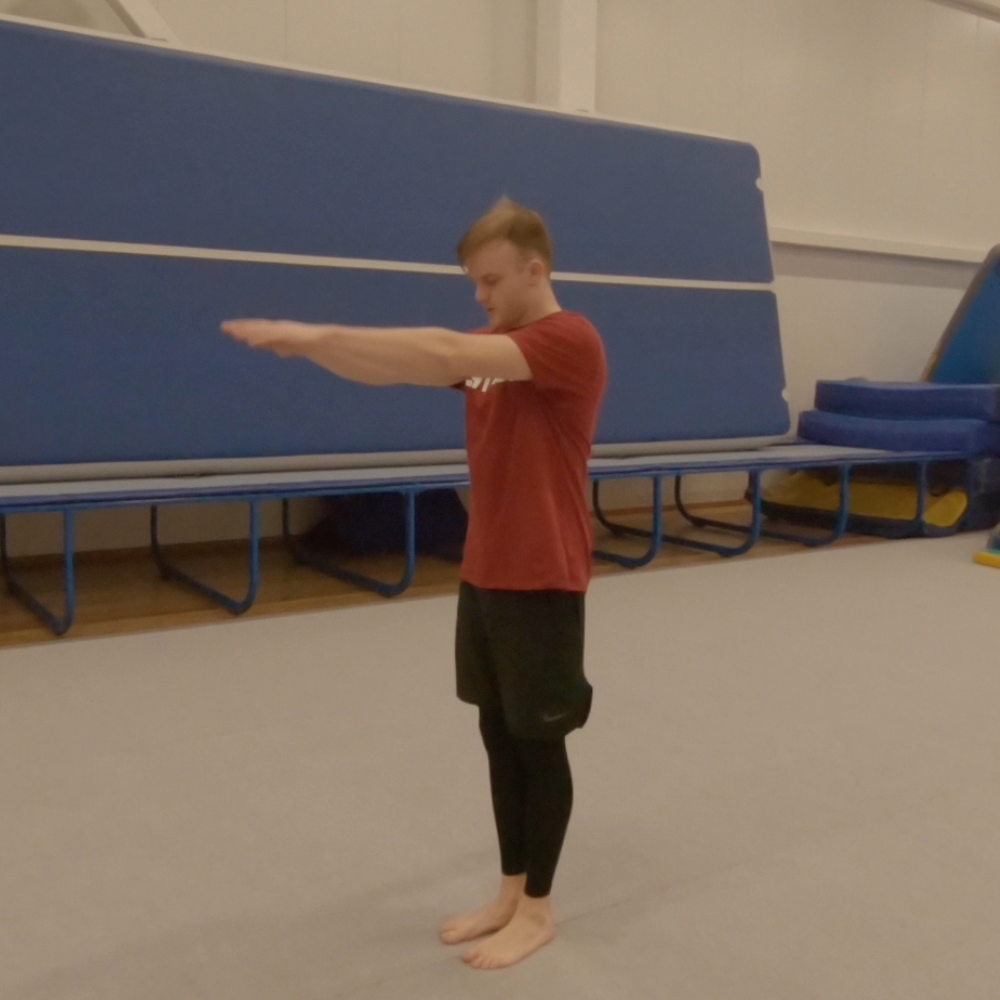
\includegraphics[width=5cm]{images/data-acquisition/example-backflip-part-1}&
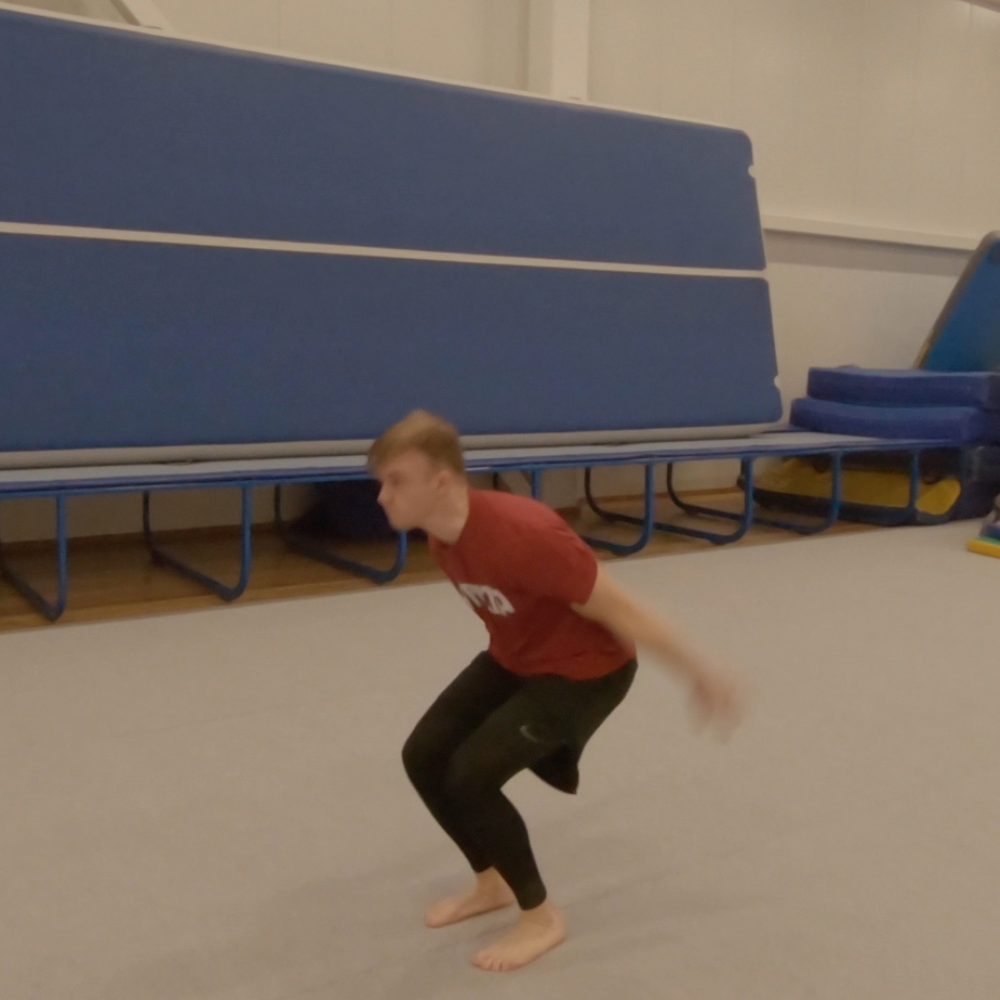
\includegraphics[width=5cm]{images/data-acquisition/example-backflip-part-2}&
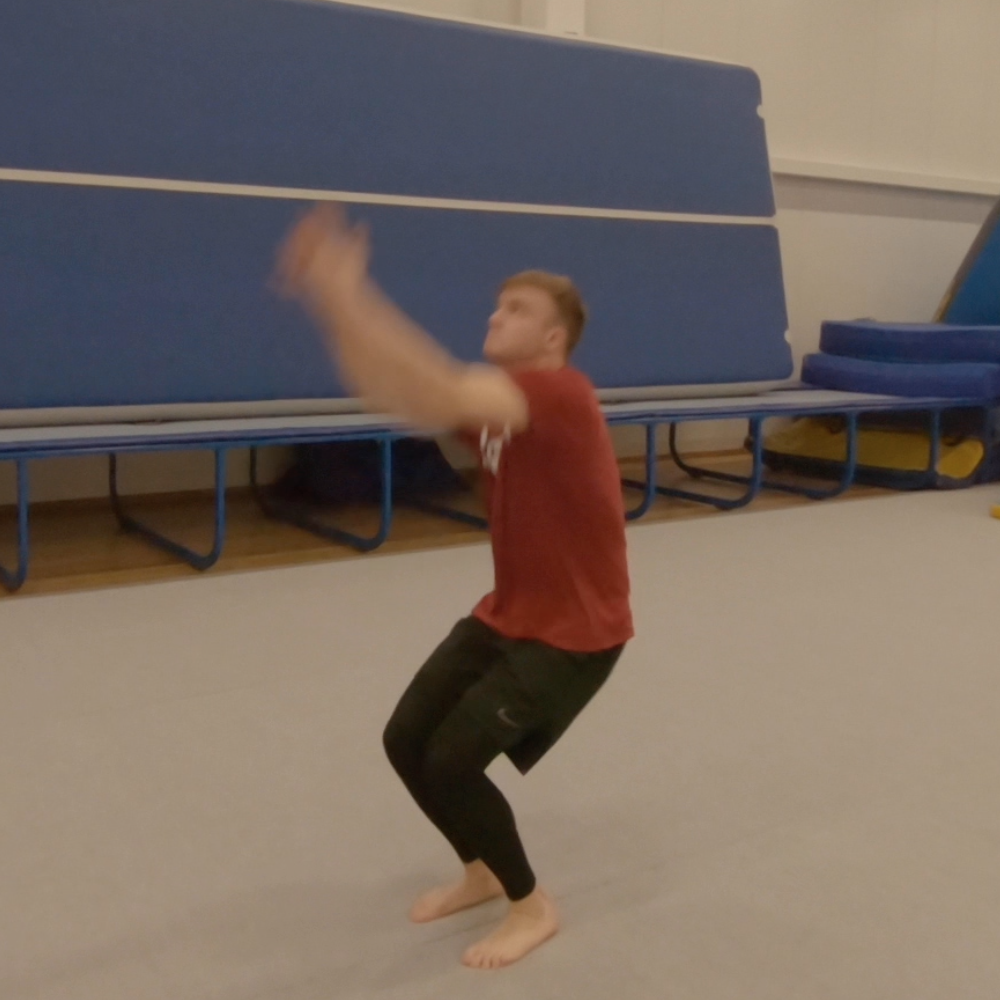
\includegraphics[width=5cm]{images/data-acquisition/example-backflip-part-3}\\
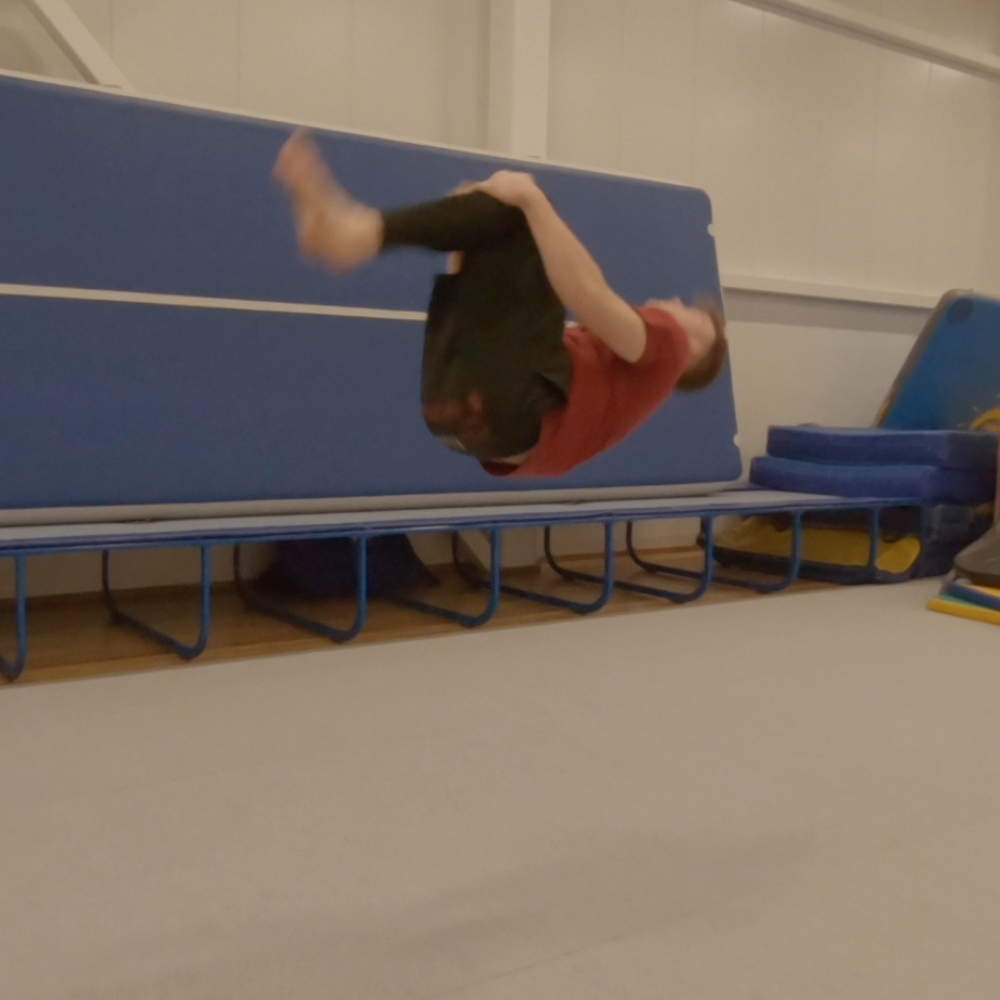
\includegraphics[width=5cm]{images/data-acquisition/example-backflip-part-4}&
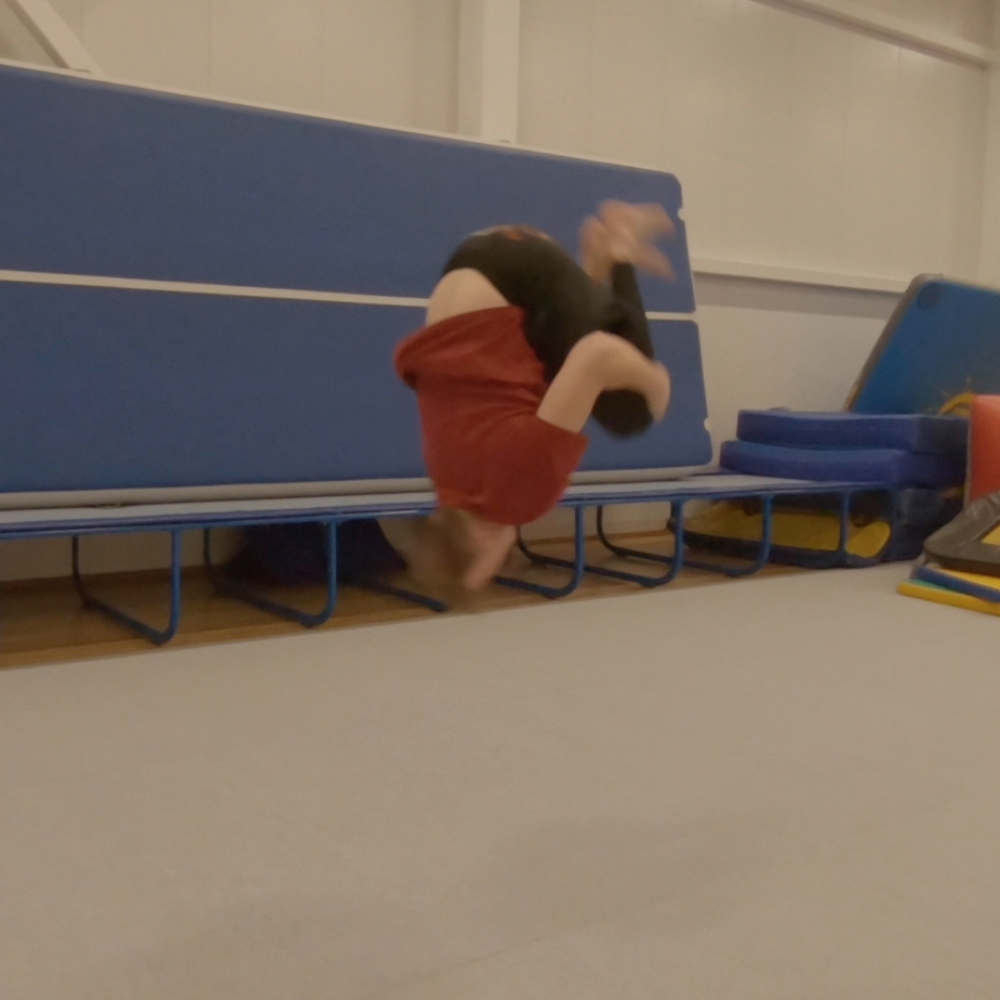
\includegraphics[width=5cm]{images/data-acquisition/example-backflip-part-5}&
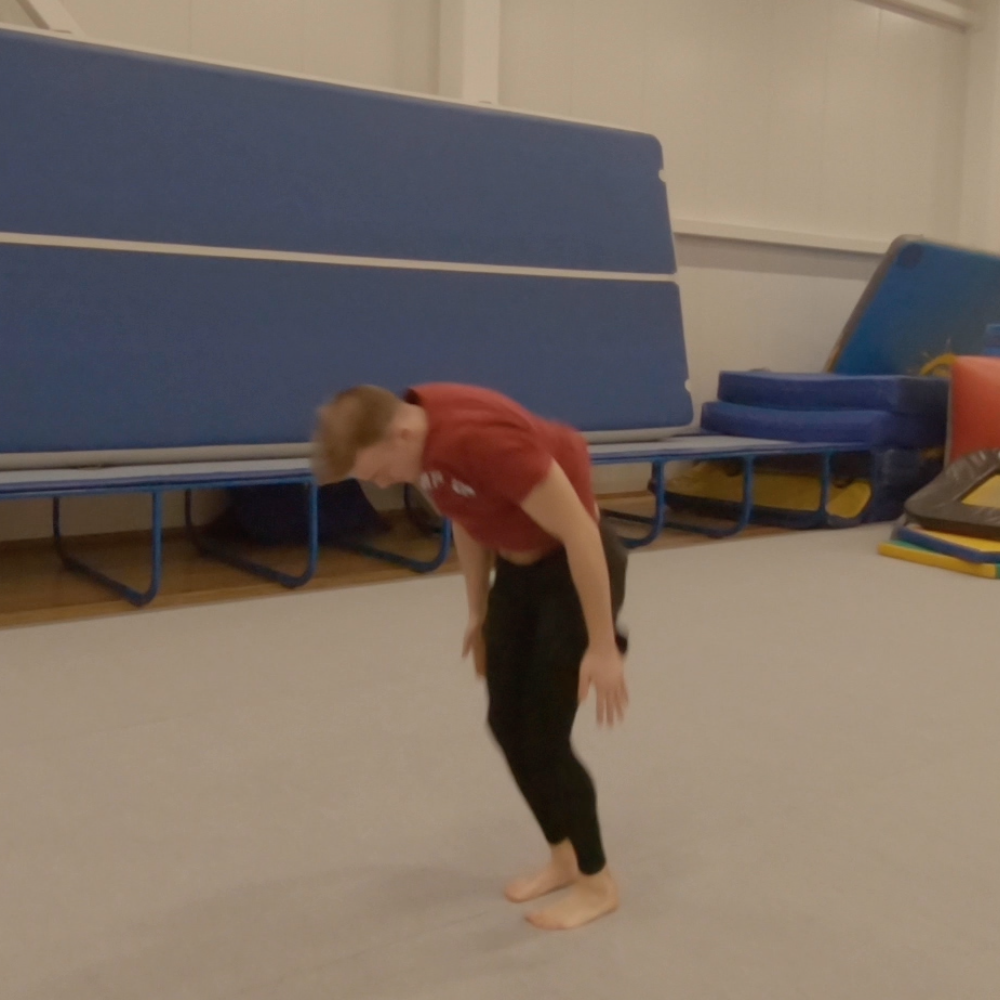
\includegraphics[width=5cm]{images/data-acquisition/example-backflip-part-6}\\
\end{tabular}
    \caption{Example of a backflip}
    \label{example-of-backflip}
\end{figure*}

\begin{figure*}
   \centering
\begin{tabular}{ccc}
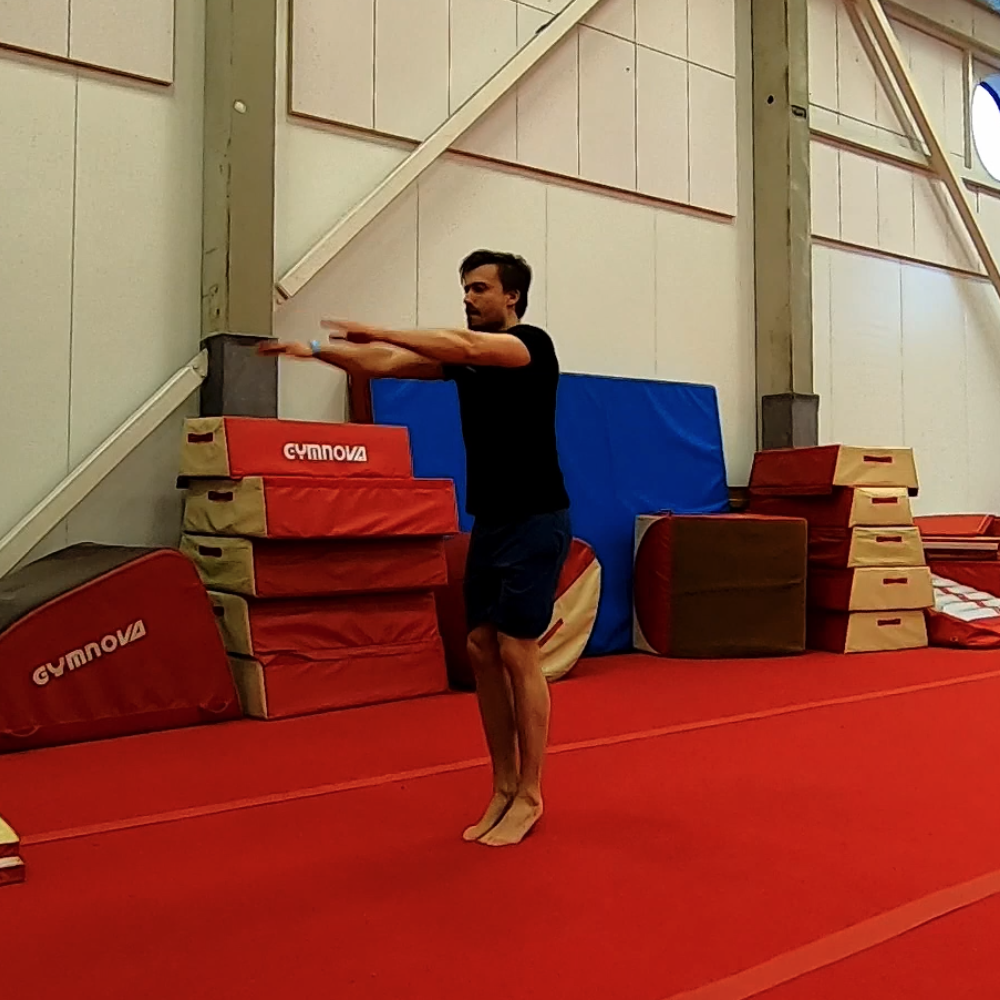
\includegraphics[width=5cm]{images/data-acquisition/example-flack-part-1}&
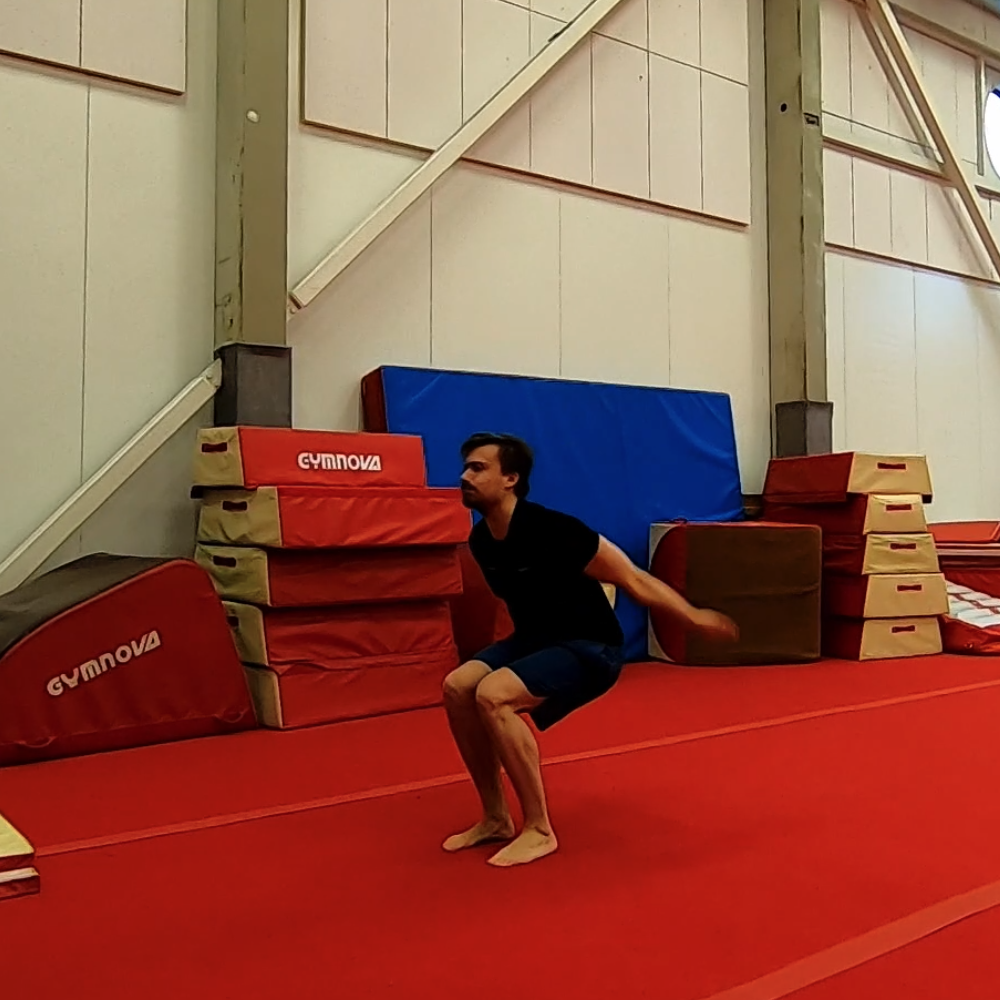
\includegraphics[width=5cm]{images/data-acquisition/example-flack-part-2}&
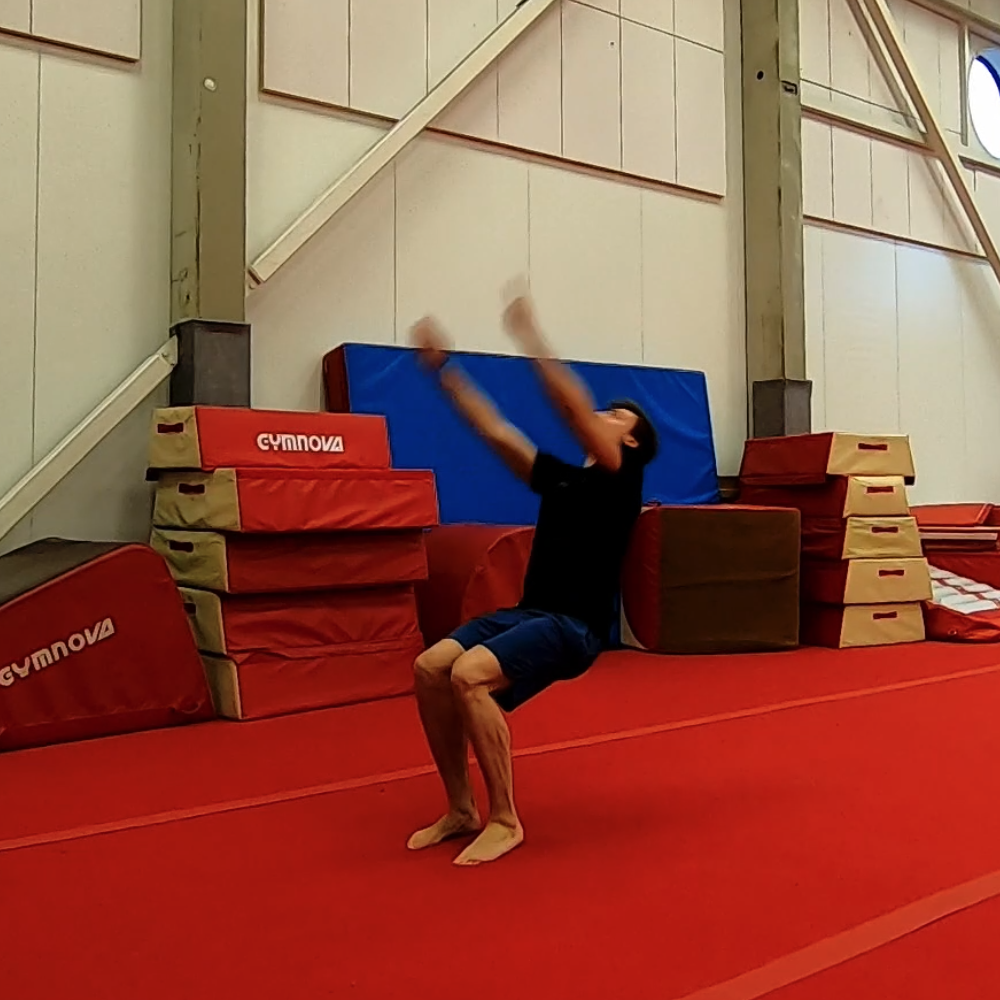
\includegraphics[width=5cm]{images/data-acquisition/example-flack-part-3}\\
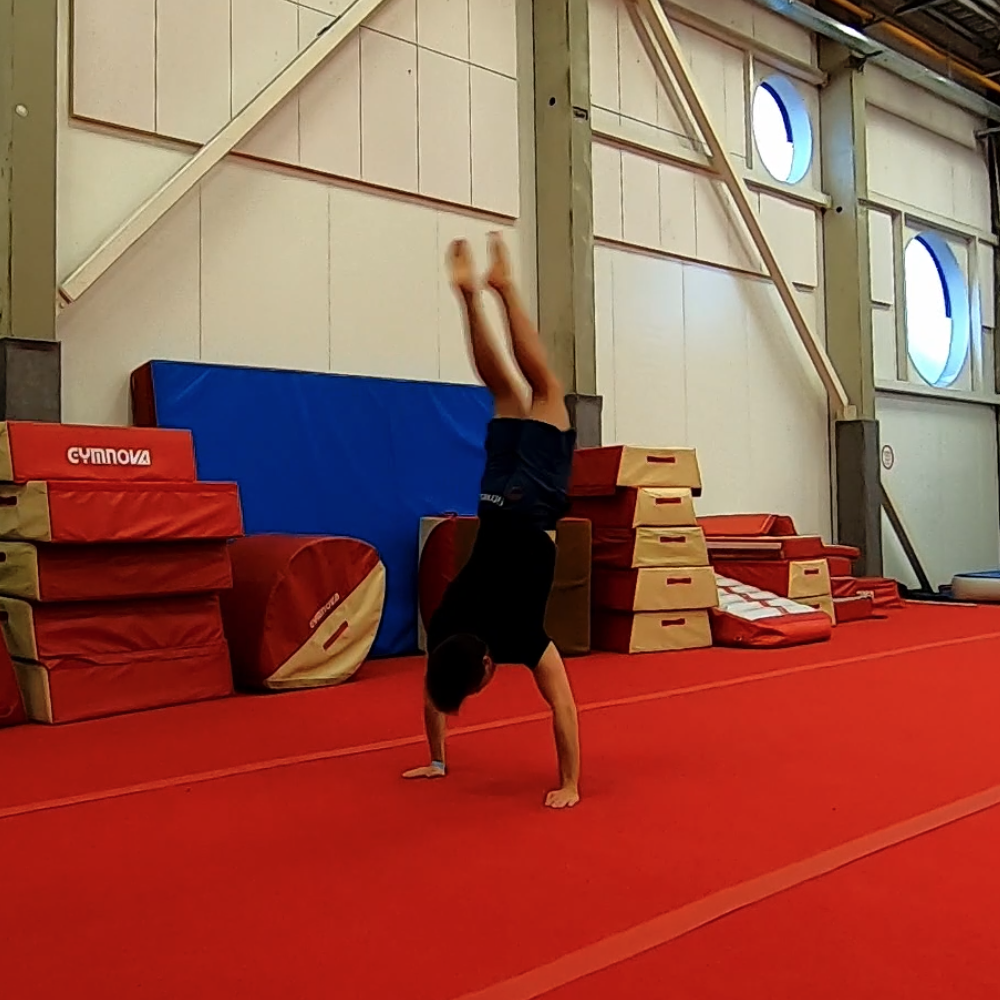
\includegraphics[width=5cm]{images/data-acquisition/example-flack-part-4}&
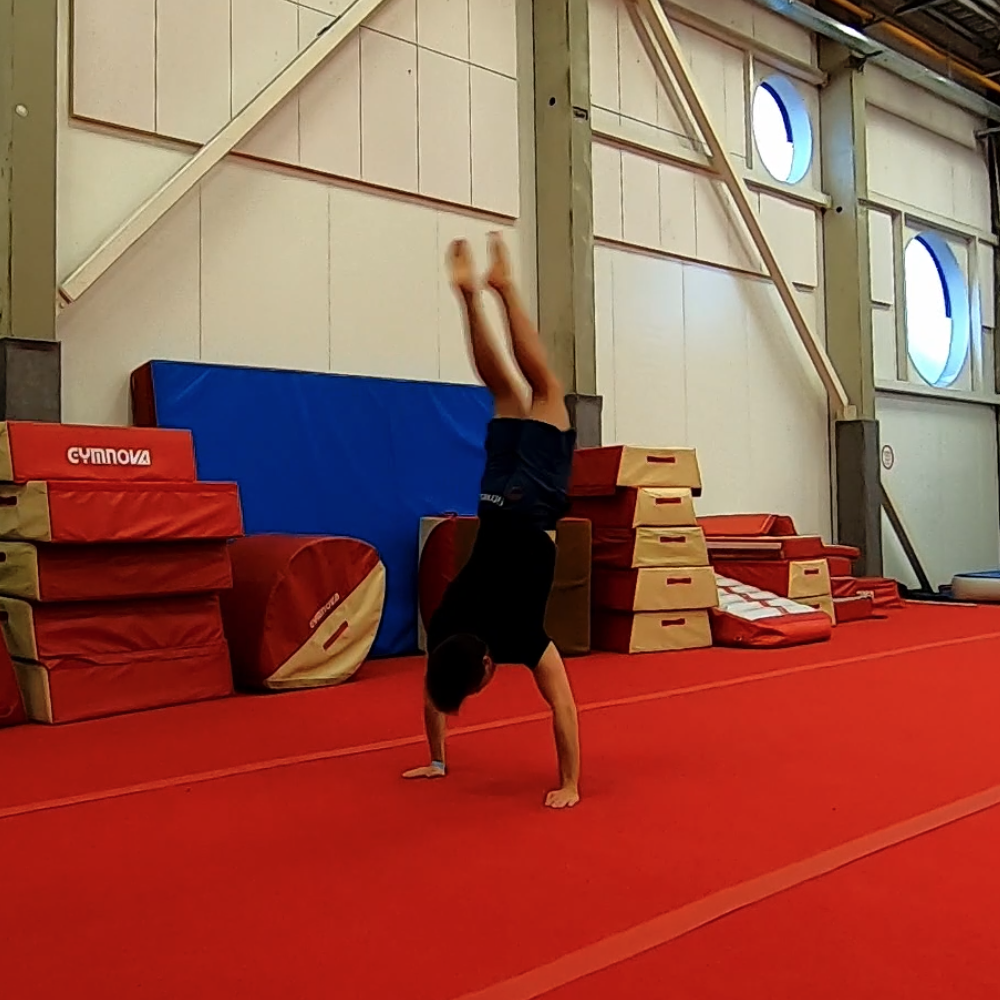
\includegraphics[width=5cm]{images/data-acquisition/example-flack-part-5}&
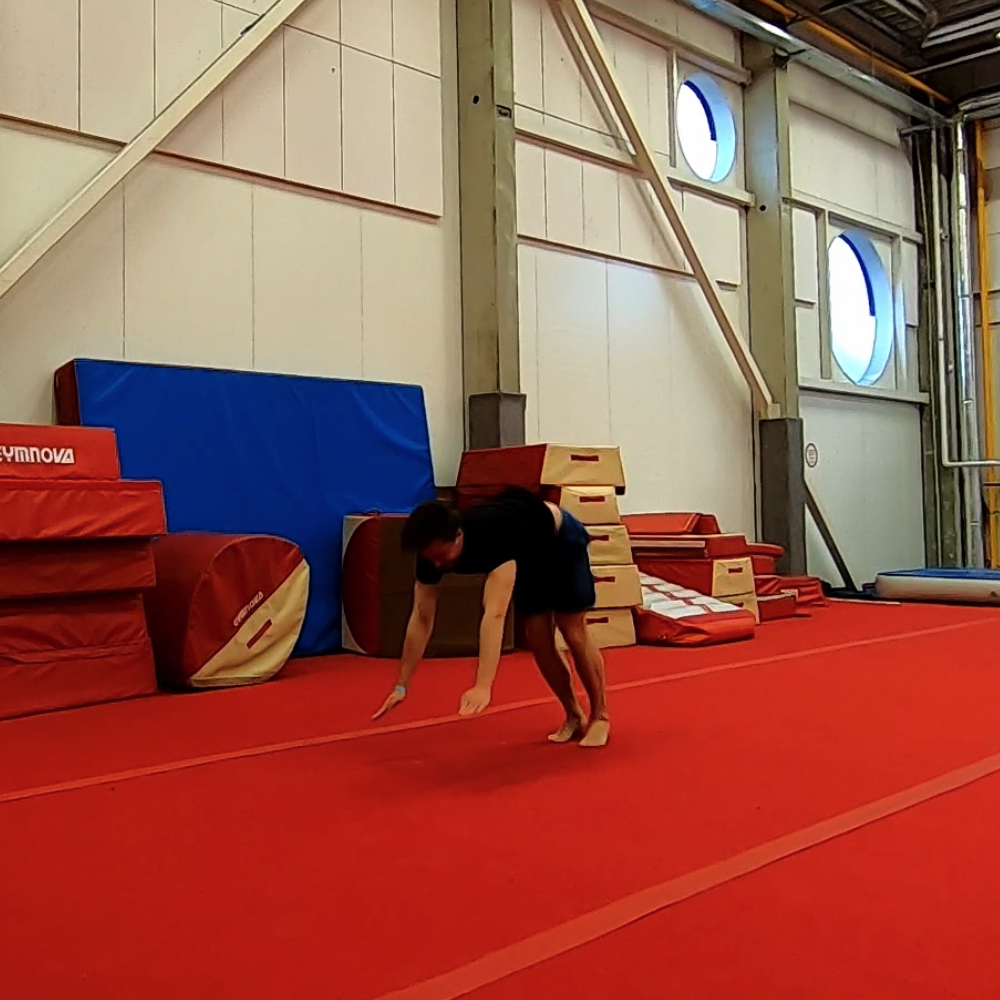
\includegraphics[width=5cm]{images/data-acquisition/example-flack-part-6}\\
\end{tabular}
    \caption{Example of a back handspring}
    \label{example-of-back-handspring}
\end{figure*}

\subsection{Identifying Activities}

As with all identifiable activities, it should be clear when the activity starts and when it ends. This paper proposes specific start and end markers for both activities, so they could be easily recognized and validated by a human observer. The markers should cover the full duration of a movement, all while sustaining the integrity and focusing on the period of interest of each activity.

A more detailed explanation of each activity and references to the visual markers can be found in sections \ref{backflip-description-section} and \ref{back-handspring-description-section}.

\subsection{Backflip}
\label{backflip-description-section}

A backflip is a sequence of body movements in which a person leaps into the air and rotates backwards over the body's horizontal axis. For the backflip, we mark the start of a backflip as the frame when athlete's both arms pass the horizontal line at shoulder level moving downwards and generating momentum. We mark the end of a backflip as the frame when both heels of the feet touch the ground again. We choose the heels of feet so we can include the amortization part of the landing phase of the backflip in the recording. The red bars in figure \ref{example-backflip-markers} demonstrate the visual markers for trimming the sample recording to include only the activity under investigation. These markers were chosen by the author to the best of his knowledge of the domain as the clearest points for a human observer to recognize a backflip. Choosing different markers is a potential discussion topic for future improvements.

\begin{figure*}
   \centering
\begin{tabular}{cc}
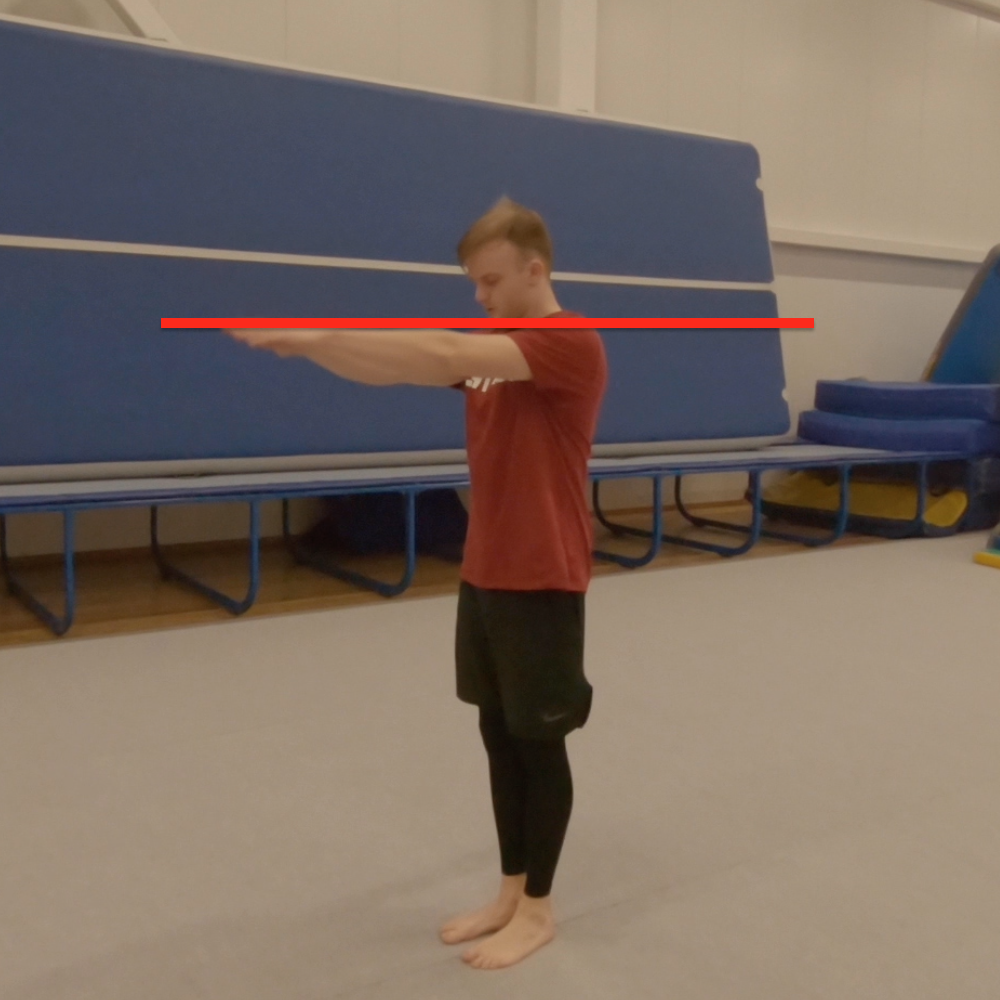
\includegraphics[width=7cm]{images/data-acquisition/example-backflip-marker-start}&
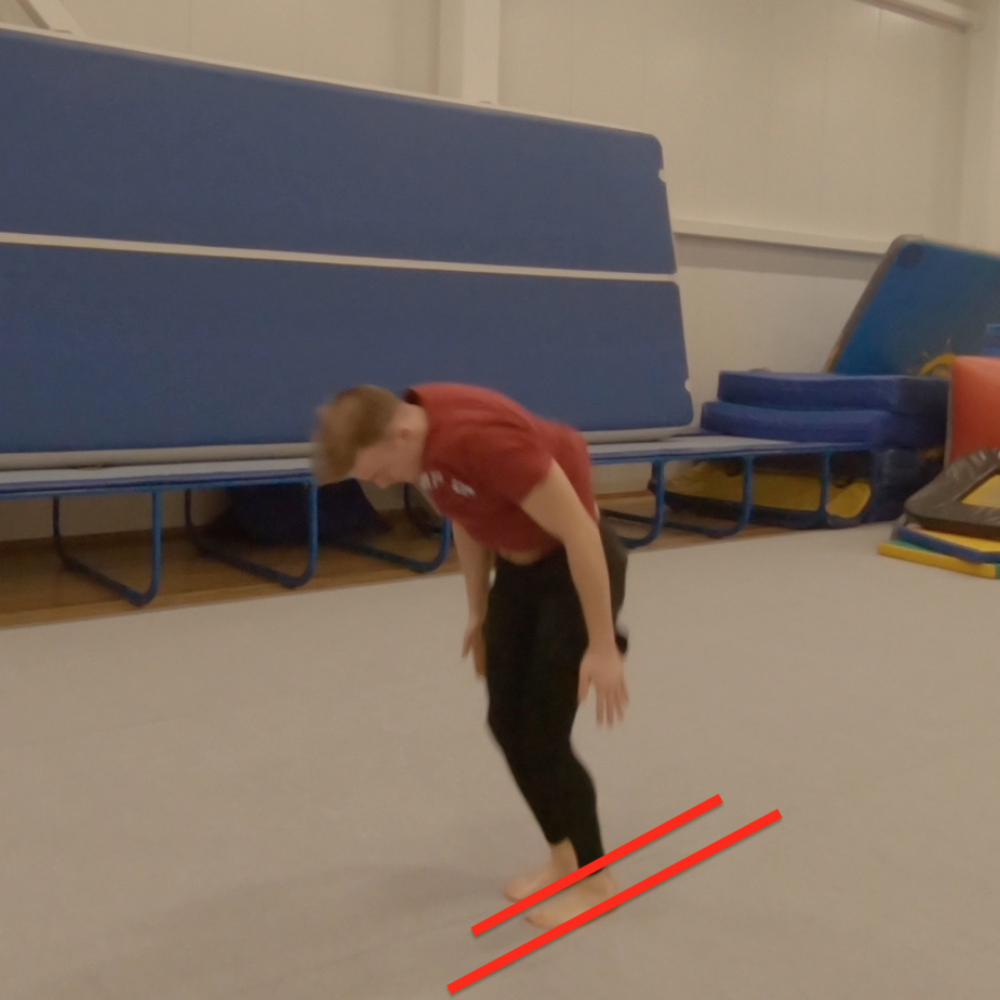
\includegraphics[width=7cm]{images/data-acquisition/example-backflip-marker-end}\\
\end{tabular}
    \caption{Start and end markers for covering the full duration of a backflip}
    \label{example-backflip-markers}
\end{figure*}

\subsection{Back Handspring}
\label{back-handspring-description-section}

A back handspring is similar to a backflip in that the athlete also rotates his body around the horizontal axis. However, during a back handspring, the athlete also moves backwards, while during a backflip the athlete should ideally not move in any direction. The other clear distinction between a back handspring and backflip is that during a back handspring, the athlete's arms extend and push off the floor to create the spring part of the activity and keep the athlete moving backwards. Thirdly, the takeoff angle differs for both back handspring and backflip. The takeoff angle decides in which direction will the athlete move during the rotation. For the backflip investigated in this paper, the goal of the athletes was to keep the takeoff angle as perpendicular as possible to the floor to keep the athlete from moving either backwards or frontwards during the rotation. However, for the back handspring, the takeoff angle should be around 45$^{\circ}$ backwards to the floor, to help the athlete move backwards and land on the hands. The green bars in figure \ref{example-back-handspring-markers} demonstrate the visual markers for covering the full duration of a back handspring. The color of markers are in both cases irrelevant and are chosen primarily for better visual distinction.

\begin{figure*}
   \centering
\begin{tabular}{cc}
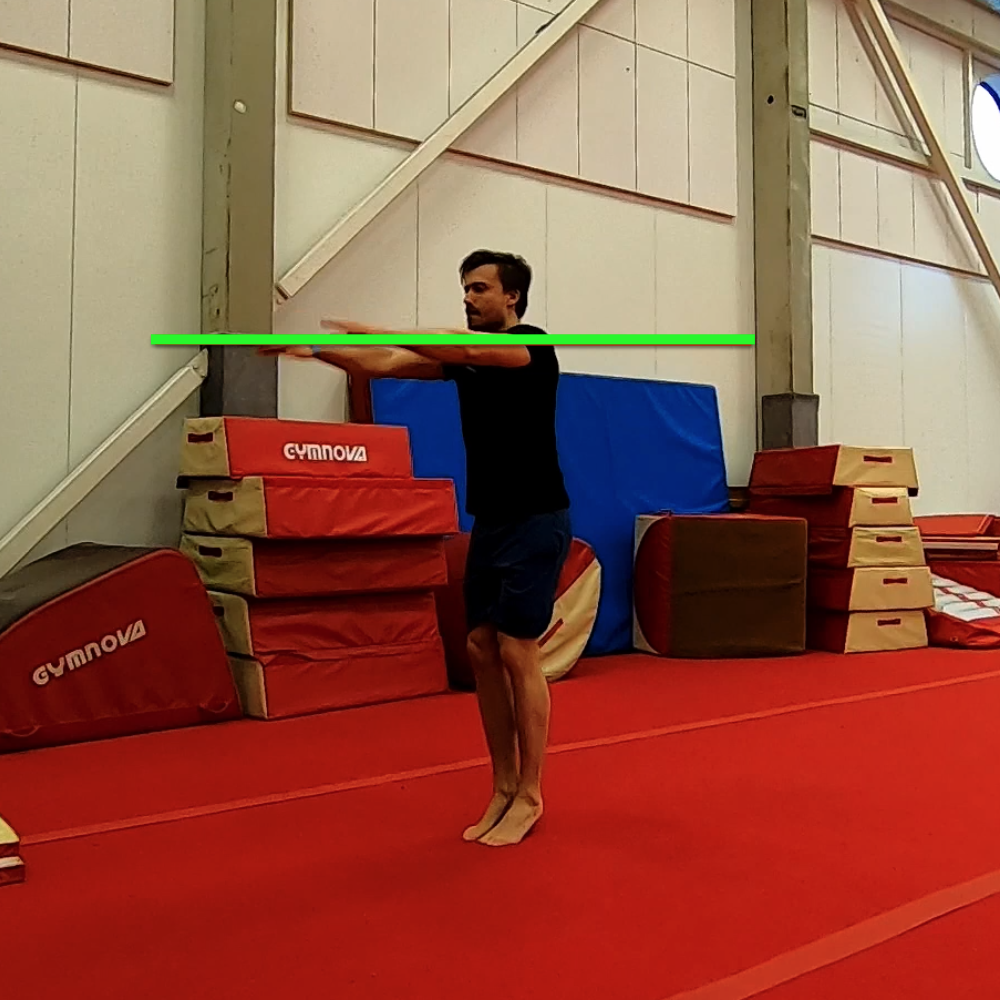
\includegraphics[width=7cm]{images/data-acquisition/example-flack-marker-start}&
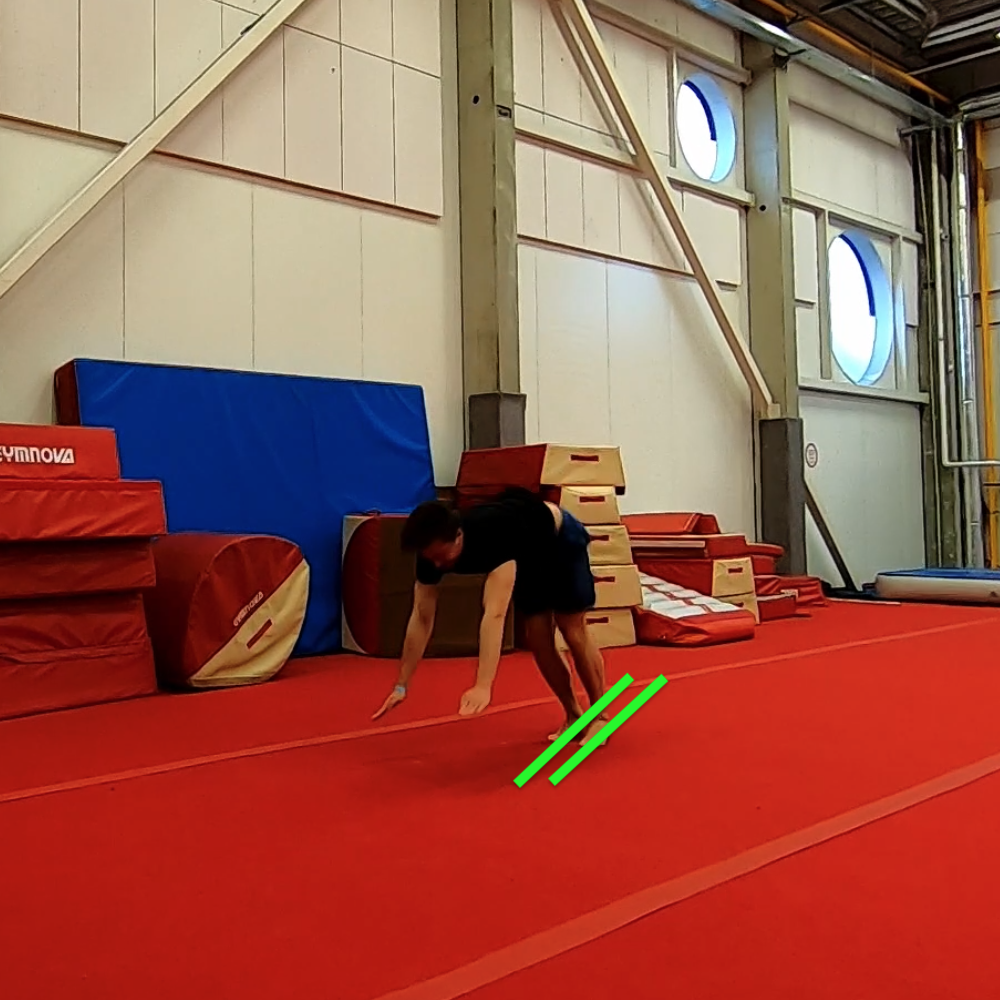
\includegraphics[width=7cm]{images/data-acquisition/example-flack-marker-end}\\
\end{tabular}
    \caption{Start and end markers for covering the full duration of a back handspring}
    \label{example-back-handspring-markers}
\end{figure*}

\subsection{Recording Process}

Since these types of movements are performed for a duration of time, just still images of activities are not sufficient. We need the activities recorded in some kind of motion picture format. The device used to capture activities is a GoPro Hero7 Black, with the following basic settings:

\begin{easylist}[itemize]

& \textit{RES} --- 1080
& \textit{FPS} --- 60
& \textit{FOV} --- Linear
& \textit{Low Light} --- Auto
& \textit{Stabilization} --- Auto
& \textit{Protune} --- Off

\end{easylist}


Each activity is recorded as one still view from eye level angle fully showing the subjects body from head to toe.

\section{Estimating and Collecting Human Action Poses}
\label{estimating-and-collecting-human-action-poses}















